% The packages used here are just a sample. You may need others, and may not need some of these. It doesn't hurt to leave them in, unless they start to conflict with other packages you've added. Chapter 2 has example code for equations, figures, tables, citations, abbreviations, etc. If there are sections labeled 'optional' that you don't want, just comment them out. -jg

\documentclass[reqno,12pt,oneside]{report} % right-side equation numbering, 12 point font, print one-sided 
%\documentclass[reqno,12pt,twoside,openright]{report} % right-side equation numbering, 12 point font, print two-sided, Chapters start on odd pages. Rackham only accepts one-sided, so this is for personal printings.

\usepackage{rac}         % Use Rackham thesis style file
\usepackage{aas_macros}  % To allow the reading of ADS journal references in the bibliography
%\usepackage[intlimits]{amsmath} % Puts the limits of integrals on top and bottom
\usepackage{amsxtra}     % Use various AMS packages
\usepackage{amsthm}
\usepackage{amssymb}
\usepackage{amsfonts}
\usepackage{graphicx}    % Add some packages for figures. Read epslatex.pdf on ctan.tug.org
\usepackage{rotating}
\usepackage{color}
\usepackage{epsfig}
\usepackage{subfigure}   % To make subfigures. Read subfigure.pdf on ctan.tug.org
%\usepackage{caption}
%\usepackage{subcaption}
\usepackage{verbatim}
\usepackage{natbib}      % Allows you to use BibTeX
\usepackage[printonlyused]{acronym} % For the List of Abbreviations. Read acronym.pdf on ctan.tug.org
\usepackage{setspace}    % Allows you to specify the line spacing
\newcommand{\fixme}[1]{\textbf{\textcolor{red}{[Fixme: #1]}}}
\newcommand{\NVDisk}{{\em NVRAM Disk-Rep\-lace\-ment}\xspace}
\newcommand{\InPlace}{{\em In-Pl\-ace Up\-dat\-es}\xspace}
\newcommand{\GroupCommit}{{\em NVRAM Group Com\-mit}\xspace}

\usepackage{textcomp}
\usepackage{txfonts}
\usepackage{booktabs}
\usepackage{multirow}

%\doublespacing           % \onehalfspacing for 1.5 spacing, \doublespacing for 2.0 spacing.
\onehalfspacing
%\newcommand{\sun}{\ensuremath{\odot}} % sun symbol is \sun
%%%%%%%%%%%%%%%%%%%%%%%%%%%%%%%%%%%%%%%%%%%%%%%%%%%%%%%%%%%%%%%%%%%%%%%%%%%%%%%

% Various theorem environments. All of the following have the same numbering
% system as theorem.

\theoremstyle{plain}
\newtheorem{theorem}{Theorem}
\newtheorem{prop}[theorem]{Proposition}
\newtheorem{corollary}[theorem]{Corollary}
\newtheorem{lemma}[theorem]{Lemma}
\newtheorem{question}[theorem]{Question}
\newtheorem{conjecture}[theorem]{Conjecture}
\newtheorem{assumption}[theorem]{Assumption}

\theoremstyle{definition}
\newtheorem{definition}[theorem]{Definition}
\newtheorem{notation}[theorem]{Notation}
\newtheorem{condition}[theorem]{Condition}
\newtheorem{example}[theorem]{Example}
\newtheorem{introduction}[theorem]{Introduction}

\theoremstyle{remark}
\newtheorem{remark}[theorem]{Remark}
%%%%%%%%%%%%%%%%%%%%%%%%%%%%%%%%%%%%%%%%%%%%%%%%%%%%%%%%%%%%%%%%%%%%%%%%%%%%%%%

\numberwithin{theorem}{chapter}     % Numbers theorems "x.y" where x
                                    % is the section number, y is the
                                    % theorem number

%\renewcommand{\thetheorem}{\arabic{chapter}.\arabic{theorem}}

%\makeatletter                      % This sequence of commands will
%\let\c@equation\c@theorem          % incorporate equation numbering
%\makeatother                       % into the theorem numbering scheme

%\renewcommand{\theenumi}{(\roman{enumi})}

%%%%%%%%%%%%%%%%%%%%%%%%%%%%%%%%%%%%%%%%%%%%%%%%%%%%%%%%%%%%%%%%%%%%%%%%%%%%%%

% If printing two-sided, this makes sure that any blank page at the 
% end of a chapter will not have a page number. 
\makeatletter
\def\cleardoublepage{\clearpage\if@twoside \ifodd\c@page\else
\hbox{}
\thispagestyle{empty}
\newpage
\if@twocolumn\hbox{}\newpage\fi\fi\fi}
\makeatother 

%%%%%%%%%%%%%%%%%%%%%%%%%%%%%%%%%%%%%%%%%%%%%%%%%%%%%%%%%%%%%%%%%%%%%%%%%%%%%%

%This command creates a box marked ``To Do'' around text.
%To use type \todo{  insert text here  }.

\newcommand{\todo}[1]{\vspace{5 mm}\par \noindent
\marginpar{\textsc{To Do}}
\framebox{\begin{minipage}[c]{0.95 \textwidth}
\tt\begin{center} #1 \end{center}\end{minipage}}\vspace{5 mm}\par}

%%%%%%%%%%%%%%%%%%%%%%%%%%%%%%%%%%%%%%%%%%%%%%%%%%%%%%%%%%%%%%%%%%%%%%%%%%%%%%%
\begin{document}

\bibliographystyle{agu04}    % Set the bibliography style. agu04, plain, alpha, etc.

% Title page as required by Rackham dissertation guidelines
\titlepage{Thesis Proposal: Database and System Design for Emerging Storage Technologies}{Steven Pelley}{Doctor of Philosophy}
{Computer Science and Engineering}{2013}
{Assistant Professor Thomas F. Wenisch, Chair\\
 Professor Peter M. Chen\\
 Assistant Professor Michael J. Cafarella\\
 Assistant Professor Zhengya Zhang}

% Begin the front matter as required by Rackham dissertation guidelines
\initializefrontsections

% Optional Frontispiece
%\frontispiece{
\includegraphics[width=6in]{Intro/Happy} Find a cool picture to go here.}

% Optional, but recommended, Copyright page
%\copyrightpage{Steven Pelley}

% Page numbering. If you don't include a frontispiece or copyright page, you'll need to change this for two-sided printing.
\makeatletter
\if@twoside \setcounter{page}{4} \else \setcounter{page}{0} \fi
\makeatother
 
% Optional Dedication page
%\dedicationpage{For all the people}

% Optional Acknowledgements page
%\startacknowledgementspage
%Thanks to the people who made this dissertation possible, especially those who put together a nice \LaTeX\, template for me to use.
%\label{Acknowledgements}

% Optional Preface page
%\startprefacepage
%\input{Preface}
%\label{Preface}

% Table of contents, list of figures, etc.
\tableofcontents     % Required
\listoffigures       % Required if there is more than one figure
\listoftables        % Required if there is more than one table
%\listofmaps          % Required if there is more than one map
\listofappendices    % Required if there is more than one appendix
\listofabbreviations % Optional. Abbreviations should be stored in a file named abbr.tex

% Optional in-dissertation Abstract Page
\startabstractpage
{Database and System Design for Emerging Storage Technologies}{Steven Pelley}{Chair: Thomas F. Wenisch}
Emerging storage technologies offer an alternative to disk that is durable and allows faster data access.
Flash memory, made popular by mobile devices, provides block access with low latency random reads.
New nonvolatile memories (NVRAM) are expected in upcoming years, presenting DRAM-like performance alongside persistent storage.
Wheres both technologies accelerate data accesses due to increased raw speed, used merely as disk replacements they may fail to achieve their full potentials.
Flash's asymmetric read/write access (i.e., reads execute faster than writes) opens new opportunities to optimize Flash-specific access.
Similarly, NVRAM's low latency persistent accesses allow new designs for high performance failure-resistant applications.

This thesis addresses software and hardware system design for such storage technologies.
First, I investigate analytics query optimization for Flash, expecting Flash's fast random access to require new query planning.
While intuition suggests scan and join selection should shift between disk and Flash, I find that query plans chosen assuming disk are already near-optimal for Flash.
Second, I examine new opportunities for durable, recoverable transaction processing with NVRAM.
Existing disk-based recovery mechanisms impose large software overheads, yet updating data in-place requires frequent device synchronization that limits throughput.
I introduce a new design, \GroupCommit, to amortize synchronization delays over many transactions, increasing throughput at some cost to transaction latency.
Finally, I propose a new framework for persistent programming and memory systems to enable high performance recoverable data structures with NVRAM, extending memory consistency with persistent semantics to introduce \emph{memory persistency}.

\label{Abstract}

\startthechapters 
% The individual files for each of the chapters are put here.
% Save each chapter of your thesis to a seperate tex file
% and then use the \input command to include this file in your
% thesis.  For instance you can save a file to "intro.tex" and 
% then type \section{Introduction}

Data center power consumption continues to grow at an alarming pace; it is projected to reach 100 billion kWh at an annual cost of \$7.4 billion within two years \cite{EPA07}, with a world-wide carbon-emissions impact similar to that of the entire Czech Republic \cite{Mankoff08}. In light of this trend, computer systems researchers, application designers, power and cooling engineers, and governmental bodies have all launched research efforts to improve data center energy efficiency.  These myriad efforts span numerous aspects of data center design (server architecture \cite{Lefurgy03,Meisner09}, scheduling \cite{Moore06, Parolini08},  power delivery systems \cite{Fan07}, cooling infrastructure \cite{Patel02}, etc.).  However, with few exceptions, existing efforts focus narrowly on energy-efficiency of single subsystems, without considering global interactions or implications across data center subsystems. 

As sophisticated power management features proliferate, the dynamic range of data center power draw (as a function of utilization) is increasing, and interactions among power management strategies across subsystems grow more complex; subsystems can no longer be analyzed in isolation.   Even questions that appear simple on their face can become quite complicated.

Reasoning about total data center power is difficult because of the diversity and complexity of data center infrastructure.  Five distinct sub-systems (designed and marketed by different industry segments) account for most of a data center's power draw:  (1) servers and storage systems, (2) power conditioning equipment, (3) cooling and humidification systems, (4) networking equipment, and (5) lighting/physical security.  Numerous sources have reported power breakdowns \cite{EPA07,Meisner09}; Table~\ref{table::PowerDistribution} illustrates a typical breakdown today.   The first three subsystems dominate and their power draw can vary drastically with data center utilization. Cooling power further depends on ambient weather conditions around the data center facility. Even the distribution of load in each subsystem can affect power draws, as the interactions among sub-systems are non-linear
%(e.g., thermal hot spots disproportionately increase cooling requirements).

In this paper, our objective is to provide tools to the computer systems community to assess and reason about total data center power.  Our approach is two-fold, targeting both \emph{data center simulation} and \emph{abstract analytic modeling}.  First, we have collected a set of detailed power models (from academic sources, industrial white papers, and product data sheets) for each critical component of data center infrastructure, which describe power draw as a function of environmental and load parameters.  Each model describes the power characteristics of a single device (i.e., one server or computer room air handler (CRAH)) and, as such, is suitable for integration into a detailed data center simulator.  We describe how these models interact (i.e., how utilization, power, and heat flow among components) and outline the design of such a simulator. To our knowledge, we are the first to describe an integrated data center simulation infrastructure; its implementation is underway.

Although these detailed models enable data center simulation, they do not allow direct analytic reasoning about total data center power.  Individual components' power draw vary non-linearly with localized conditions (i.e., temperature at a CRAH inlet, utilization of an individual server), that require detailed simulation to assess precisely.  Hence, to enable back-of-the-envelope reasoning, we develop an \emph{abstract model} that replaces key steps of the data center simulation process with simple parametric models that enable analysis of average behavior.  In particular, we abstract away time-varying scheduling/load distribution across servers and detailed tracking of the thermodynamics of data center airflow.  Our abstract model provides insight into how data center sub-systems interact and allows quick comparison of energy-efficiency optimizations.

\begin{table}[t]
\begin{center}
\caption{ \textbf{Typical Data Center Power Breakdown.} }
\label{table::PowerDistribution}

\begin{tabularx}{\linewidth}{c c c c c}
    \toprule
    Servers & Cooling & Power Cond. & Network & Lighting \\
    \midrule
    56\% & 30\% & 8\% & 5\% & 1\% \\
    \bottomrule
  \end{tabularx}
\end{center}

\end{table}
. 

 \chapter{Introduction}
 \label{chap:Intro}
 For decades disk has been the primary technology for durable and large-capacity storage.
Although inexpensive and dense, disk provides high performance only for coarse-grained sequential access and suffers enormous slowdowns for random reads and writes.
Recently, several new technologies have emerged as popular or viable storage alternatives.
Flash memory, primarily used for mobile storage, has gained traction as a high-performance enterprise storage solution.
Nonvolatile Random Access Memories (NVRAM), such as phase change memory and spin-transfer torque RAM, have emerged as high performance storage alternatives \cite{BurrKurdi08}.

These technologies offer significant performance improvements over disk, while still providing durability with great storage capacity.
As drop-in replacements for disk, Flash and NVRAM greatly accelerate storage access.
However, the disk interface fails to leverage specific device characteristics.
Section~\ref{sec:Background:Storage} provides a background on these storage technologies and specifically how their performance differs from disk.

This dissertation investigates how several data-centric workloads interact with future storage technologies, the relevant software and algorithms, and in some instances computer hardware.
Specifically, I consider analytics (commonly Decision Support Systems -- DSS -- popular in ``Big Data") and On-Line Transaction Processing (OLTP).
Both workload classes have been optimized to surmount disk's constraints, yet storage devices often remain the performance bottleneck and dominant cost.
I match each workload to the emerging storage technology that suits it best and address specific opportunities or deficiencies in the software and hardware systems.

\section{Analytics}
\label{sec:Intro:Analytics}

Analytics relies on disk to provide enormous data capacity.
Typical analytics work-flow involves taking a snapshot of data from an online database and mining this data for complex, yet useful, patterns.
While applications do not rely on disk's durability for recovery (in fact, instances that fit in main memory have no need for disk), modern analytics data sets reach peta-byte scale \cite{Economist10}, and accessing such large data imposes the dominant bottleneck.
Such capacity is currently achieved only by dense disk and Flash memory.

Decades of research have provided modern analytics databases with tools to minimize storage accesses, particularly slow random accesses (e.g., disk-specific indexes, join algorithms to minimize page access and produce large sequential runs).
Whereas these optimizations are still effective for Flash, they fail to leverage Flash's ability to quickly read non-sequential data (many optimizations purposefully avoid random access patterns on disk).
As examples, I consider access paths (various scan types) and join algorithms.
An historic rule of thumb for scans is that an index should be used when less than 10\% of rows in a table are returned, otherwise the entire table should be scanned \cite{RamakrishnanAndGehrke}.
The intuition is that locating rows from an index requires random reads as well as reading additional pages from the index itself.
At sufficiently high selectivities, accessing the entire table, scanning all rows and returning those that satisfy the query, provides a faster access path.
One would expect this selectivity (10\%) to increase when replacing disk with Flash -- Flash is no longer penalized by random reads, preferring any scan that minimizes total page accesses.
Similarly, different ad hoc join algorithms (those that do not use indexes: block-nested loops, sort-merge join, and hybrid-hash join) present different storage access patterns and may be variably suited to disk and Flash.
These algorithms and query optimization are further discussed in Section~\ref{sec:Background:Scans}.

My results, originally presented in ADMS 2010 \cite{PelleyWenisch11} and discussed in Chapter~\ref{chap:FlashOpti}, show that while both previous hypotheses are correct, their significance is negligible.
Optimal access path (index vs. table scan) only changes between disk and Flash for a small range of query selectivities, and queries within that range see only a small performance improvement.
Additionally, join algorithm choice makes little difference, as optimized join algorithms already minimize storage accesses, regardless of access pattern---join algorithms optimized for disk are already optimized for Flash.
I conclude that the page-oriented nature of Flash limits further analytics-Flash optimization.
On the other hand, emerging byte-addressable NVRAMs offer finer-grained access.
However, analytics does not require persistent storage, instead using NVRAM as a replacement for DRAM.
As DRAM-resident analytics techniques are already well established, I instead investigate using NVRAM persistence specifically to provide failure recovery, supporting durable transactions.

\section{Transaction Processing}
\label{sec:Intro:OLTP}

Databases have been designed for decades to provide high-throughput transaction processing with disk.
Write Ahead Logging (WAL) techniques, such as ARIES \cite{MohanHaderle92}, transform random writes into sequential writes and minimize transactions' dependences on disk accesses.
Section~\ref{sec:Background:Recovery} outlines modern recovery management, focusing on ARIES.
With sufficient device throughput (IOPS) and read-buffering, databases can be made compute-bound and recover near-instantly.
NVRAMs provide this massive storage throughput to the masses.

Whereas ARIES is necessary for disk, it presents only unnecessary software overheads to NVRAM.
I show that removing ARIES improves transaction throughput by alleviating software bottlenecks inherent in centralized logging.
Instead, NVRAM allows data to be updated in-place, enforcing data persistence immediately and providing correct recovery via transaction-local undo logs.

NVRAMs, however, are not without their limitations.
Se\-veral candidate NVRAM technologies exhibit larger read latency and significantly larger write latency compared to DRAM \cite{BurrKurdi08}.
Additionally, whereas DRAM writes benefit from caching and typically are not on applications' critical paths, NVRAM writes must become persistent in a constrained order to ensure correct recovery.
I consider an NVRAM access model where correct ordering of persistent writes is enforced via \emph{persist barriers}, which stall until preceding NVRAM writes complete; such persist barriers introduce substantial delays when NVRAM writes are slow.

To address these challenges I investigate accelerating NVRAM reads with various cache architectures and capacities, and avoid persist barrier delays by introducing a new recovery mechanism, \GroupCommit.
Database designs are discussed in Chapter~\ref{chap:OLTP_design}.
As expected, low latency memory-bus-connected NVRAM needs little additional caching (on-chip caches suffice) and updating data in-place is a simple and viable recovery strategy.
However, long latency NVRAM and complex interconnects (e.g., Non-Uniform Memory Architectures -- NUMA, PCIe-attached NVRAM, or distributed storage) benefit from DRAM caching and \GroupCommit, improving throughput.
I investigate specifically how NVRAM read and persist barrier latencies drive OLTP system design.
These results and additional evaluations are presented in Chapter~\ref{chap:OLTP_eval}.
This work was originally published at VLDB \cite{Pelley13}.

\section{Memory Persistency}
\label{sec:Intro:PMC}

The previous work looks at how OLTP recovery mechanisms should be designed, considering only the average delay incurred by persist barriers.
The final portion of my dissertation investigates specific programming interfaces to order NVRAM writes.
Whereas existing memory consistency models provide control over the order and visibility of volatile memory reads and writes across threads, there are no equivalent models to reason about data persistence.
Memory consistency may be relaxed, allowing communicating threads to each observe different memory read and write orders.
Such memory consistency models improve performance, but require complex reasoning and additional programming mechanisms (memory barriers) to ensure expected behavior.
Memory models are described in Section~\ref{sec:Background:MemoryConsistency}.

Similarly, NVRAM write order may be relaxed, improving performance by allowing writes to occur in parallel or out of order while still ensuring correct recovery.
I introduce \emph{memory persistency}, a framework that extends memory consistency, to reason about NVRAM write order.
Relaxed memory persistency models use persist barriers to enforce specific write orders, guaranteeing that data is correctly recovered after failure.
I define memory persistency and enumerate the possible design space in Chapter~\ref{chap:Persistency}.
Interestingly, memory persistency models may be de-coupled from the underlying memory consistency models, separately enforcing the order in which writes become durable and the order in which writes become visible to other threads.
I introduce a persistent queue benchmark and several memory persistency models in Chapter~\ref{chap:PersistencyModels}.
Finally, I evaluate these models in Chapter~\ref{chap:PersistencyEval}.
Strict persistency models slow execution nearly $30\times$ relative to existing throughput on volatile, nonrecoverable systems.
Relaxed persistency models regain lost throughput by improving NVRAM write concurrency.

\section{Data Center Infrastructure}
\label{sec:Intro:Additional}
The themes of this dissertation include performance, cost efficiency, and reliability.
While I focus on storage architectures, I additionally published work regarding the cost and reliability of data center infrastructure.
Appendix~\ref{app:WEED} contains ``Understanding and Abstracting Total Data Center Power," published at WEED 2009 \cite{PelleyMeisner09}.
This work presents power/energy models for all aspects of the data center, including power distribution, battery backups, cooling infrastructure, and IT equipment.
Appendix~\ref{app:PowerRouting} contains ``PowerRouting: Dynamic Power Provisioning for the Data Center," published at ASPLOS 2010 \cite{PelleyMeisner10}.
PowerRouting spreads power distribution responsibility throughout the data center to minimize installed power infrastructure capacity while maintaining reliability, minimizing data center cost.
The key insight is that data centers typically over-provision infrastructure, resulting in under-utilized (and often unnecessary) equipment.
PowerRouting leverages compute-specific knowledge of the IT workload to more effectively utilize power infrastructure.
Both of these works are included without modification.

During my investigations I discovered that, in many regards, industry is ahead of academia at decreasing operating costs and improving infrastructure efficiency.
As such, the opportunity to contribute meaningful new techniques to improve infrastructure is rapidly diminishing.
Recognizing storage and memory as primary concerns for energy efficiency, reliability, and cost, I focus on new and emerging storage technologies in this dissertation.

\section{Summary}
\label{sec:Intro:Summary}
This dissertation investigates new techniques for accelerating data access for new NVRAM storage technologies, and is organized as follows:
Chapter~\ref{chap:Background} contains background information on storage technologies, database optimizations, and memory consistency.
This background forms the foundation of the work that follows.
Chapter~\ref{chap:FlashOpti} considers taking advantage of Flash's fast random reads to accelerate database analytics.
In Chapter~\ref{chap:OLTP_design}, I describe potential software designs for OLTP using NVRAM.
Chapter~\ref{chap:OLTP_eval} details a methodology to evaluate NVRAM (devices not readily available) on modern hardware and evaluates several aspects of OLTP running on NVRAM.
Chapter~\ref{chap:Persistency} introduces and defines memory persistency.
Specific memory persistency models and a persistent queue data structure are proposed in Chapter~\ref{chap:PersistencyModels}.
Finally, I evaluate these memory persistency models in Chapter~\ref{chap:PersistencyEval}.


 \chapter{Background}
 \label{chap:Background}
 This chapter provides details necessary to understand the investigations and experiments in this thesis.
I focus on storage technologies, database analytics optimization, and database transaction processing optimizations.
The purpose of discussing database optimizations is to understand the complications that arise when using disk for large capacity or durability, and how this will interact with emerging storage technologies.

\section{Storage Technologies}
\label{sec:Background:Storage}

I start with a survey of storage technologies including disk, flash, and upcoming NVRAM.
For each, I provide the operating principles and interesting technological trends.

\begin{table}
  \centering
  \begin{tabular}{ l l l }
  %\begin{tabular}{r@{\hspace{12pt}}c@{\hspace{12pt}}c@{\hspace{12pt}}}
  \toprule
   & Disk & Flash \\
   \midrule
   Model & WD VelociRaptor 10Krpm & OCZ RevoDrive \\
   Capacity & 300gb & 120gb \\
   Price & \$164 & \$300 \\
   Random Read & 10ms & 90$\muup$s \\
   Seq. Read & 120mb/s & 190mb/s \\
  \bottomrule
  \end{tabular}

  \caption{Disk Characteristics}
  \label{table::DiskCharacteristics}
\end{table}


\subsection{Disk}
\label{sec:Background:Storage:Disk}
\todo{find some citation for disk.  System R?  Also citation for operating principles}
I provide a summary of disk here only for comparison and to be thorough.
Disk has been the primary durable and high capacity storage technology for decades.
Disks function by storing data on spinning magnetic platters.
Accessing data requires moving the \emph{hard disk head} onto the proper \emph{track}.
Once the head settles, it may read or write data once the platter rotates and the correct sector within the track reaches the head.
Disk capacity increases with the areal size and number of platters, as well as areal density (placing more sectors and tracks within the same area).
Because capacity has scaled so well (and continues to), disk remains an important technology for large datasets and persistent storage.

While dominant, disk exhibits relatively slow access and undesirable access behavior.
Rotational speed limits the rate that data transfers to or from the disk.
Further, random reads and writes must first seek to the proper track and then wait until the sector of interest reaches the head, a process which takes several ms.
Table~\ref{table:DiskCharacteristics} lists the measured performance characteristics of an enterprise disk.
My disk achieves nearly 120 MB/s sequential transfers, but random reads take an average of 10ms (only 50 KB/s for 512 byte sectors!).
As a result, there is a large history of optimization for disk-resident storage, as I discuss later in the chapter.

\subsection{Flash Memory}
\label{sec:Background:Flash}
Driven by the popularity of mobile devices, Flash memory has quickly improved in both storage density and cost to the point where it has become a viable alternative for durable storage even in enterprise-class systems.
Unlike conventional rotating hard disks, which store data using magnetic materials, Flash stores charge on a floating-gate transistor, forming a memory cell.
These transistors are arranged in arrays resembling NAND logic gates, after which the ``NAND Flash'' technology is named.
This layout gives NAND Flash a high storage density relative to other memory technologies.
Though dense, the layout sacrifices byte addressability and some read latency---an entire array (a.k.a. page, typically 2KB to 4KB) must be read in a single operation---making NAND Flash more appropriate for block-oriented IO than as a direct replacement for RAM.  

One of the difficulties of Flash devices is that a cell can be more easily programmed (by adding electrons to the floating gate) than erased (removing these electrons).  
Erase operations require both greater energy and latency, and typically can be applied only at coarse granularity (e.g., over blocks of 128KB to 512KB).
Moreover, repeated erase operations cause the Flash cell to wear out over time, limiting the maximum lifetime of the cell (e.g., to $10^5$ to $10^6$ writes \cite{Roberts2009}).  
Recent Flash devices further increase storage density by using several distinct charge values to represent multiple bits in a single cell at the cost of slower accesses and even shorter lifetimes.

A Flash-based SSD wraps an array of underlying Flash memory chips with a controller that manages capacity allocation, mapping, and wear leveling across the individual Flash devices.  
The controller mimics the interface of a conventional (e.g., SATA) hard drive, allowing Flash SSDs to be drop-in replacements for conventional disks.
      
As previously noted, Flash SSDs provide substantially better performance than disks, particularly for random reads, but at higher cost.
Table \ref{table:DiskCharacteristics} lists specifications of a typical Flash SSD as compared to a 10,000 RPM hard drive.
Though neither of these devices are the highest-performing available today, they are representative of the mid-range of their respective markets.
The latency for a random read is over 100\texttimes~better on the SSD than on the disk, while the sequential read bandwidth is 1.6\texttimes~better. 
Unlike disks, where each random read incurs mechanical delays (disk head seek and rotational delays), on SSDs, a random read is nearly as fast as a sequential read.  

\subsection{NVRAM}
\label{sec:Background:NVRAM}

Nonvolatile memories will soon be commonplace.
Technology trends suggest that DRAM and flash memory may cease to scale, requiring new dense memory technologies \cite{LeeIpek09}.

\textbf{Memory technology characteristics.}
Numerous technologies offer durable byte-addressable access.
Examples include phase change memory (PCM), where a chalcogenide glass is heated to produce varying electrical conductivities, and spin-transfer torque memory (STT-RAM), a magnetic memory that stores state in electron spin \cite{BurrKurdi08}.
Storage capacity increases by storing more than two states per cell in Multi-level Cells (MLC) (e.g., four distinct resistivity levels provide storage of 2 bits per cell).

While it remains unclear which of these technologies will eventually dominate, many share common characteristics.
In particular, NVRAMs will likely provide somewhat higher access latency relative to DRAM.
Furthermore, several technologies are expected to have asymmetric read-write latencies, where writing to the device may take several microseconds \cite{QureshiSrinivasan09}, although substantial faster than disk or flash.
Write latency worsens with MLC, where slow, iterative writes are necessary to reliably write to a cell.

Similarly to flash, resistive NVRAM technologies suffer from limited write endurance; cells may be written reliably only a limited number of times.
Previously proposed hardware mechanisms (e.g., Start-Gap \cite{QureshiKaridis09}) are highly effective in distributing writes across cells and can mitigate write endurance concerns.
While such work focuses on volatile applications (NVRAM as a DRAM main memory substitute), it may be extended to durable uses.

\textbf{NVRAM storage architectures.}
Future database systems may incorporate NVRAM in a variety of ways.
At one extreme, NVRAM can be deployed as a disk or flash SSD replacement.
While safe, cost-effective, and backwards compatible, the traditional disk interface imposes overheads.
Prior work demonstrates that file system and disk controller latencies dominate NVRAM access times \cite{CaulfieldDe10}.
Furthermore, block access negates advantages of byte addressability.

Recent research proposes alternative device interfaces for NVRAM.
Caulfield \emph{et al.} propose Moneta and Moneta Direct, a PCIe attached PCM device \cite{CaulfieldMollov12}.
Unlike disk, Moneta Direct bypasses expensive system software and disk controller hardware to minimize access latency while still providing traditional file system semantics.
However, Moneta retains a block interface.
Condit \emph{et al.} suggest that NVRAM connect directly to the memory bus, with additional hardware and software mechanisms providing file system access and consistency \cite{ConditNightingale09}.
I later adopt the same atomic eight-byte persistent write, enabling small, safe writes even in the face of failure.
NVRAM will eventually connect via a memory interface, but it is unclear how NVRAM storage will evolve or what its exact performance characteristics will be.

\section{Analytics Optimization}
\label{sec:Background:Analytics}

Large scale data processing requires efficient use of storage devices.
I discuss two important operators within the relational model most affected by flash's performance characteristics: scans and joins.

\subsection{Scans}
\label{sec:Background:Scans}

Whenever a query accesses a table, the query optimizer must choose an access path for that table. 
The goal is to select all relevant rows from the table while touching the least number of storage pages, frequently with the use of indexes.
Work on access path selection dates back to the late 1970s \cite{Selinger1979}.
There are two classic scan operators implemented by nearly all commercial DBMS systems: \emph{relation scan} and \emph{index scan}.
An index is a database data structure that maps values within a row back to that row.
Additionally, indexes may be ordered (as in an in-memory balanced tree or disk-resident B-Tree) to efficiently retrieve all rows satisfying a range query (e.g., an ordered index on ``last name" would accelerate a query asking for all people whose last name is between ``Pelley" and ``Wenisch").
Many types of indexes exist, but all that must be considered here is that they provide a more direct way to filter specific data than scanning an entire data set.

When no indexes are available, the only choice is to perform a \emph{relation scan}, where all data pages in the table are read from disk and scanned tuple-by-tuple to select relevant tuples.
When a relevant index is available, the DBMS may instead choose to perform an \emph{index scan}, where the execution engine traverses the relevant portion of the index and fetches only pages containing selected tuples as needed.

For clustered indexes (i.e., the row itself exists within the index, and all rows are sorted according to the index key), an index scan is nearly always the preferred access path, regardless of the underlying storage device.  
For non-clustered indexes, whether the optimizer should choose a relation scan or index scan depends on the selectivity of the query; relation scans have roughly constant cost regardless of selectivity, whereas index scan costs grow approximately linearly with selectivity.
When selectivity is low, the index scan provides greater performance because it minimizes the total amount of data that must be transferred from disk.
However, as selectivity increases, the fixed-cost relation scan becomes faster.  
Though the relation scan reads the entire table, it can do so using sequential rather than random IO, leveraging the better sequential IO performance of rotating hard disks.
A classic rule of thumb for access path selection is to choose a relation scan once selectivity exceeds ten percent \cite{RamakrishnanAndGehrke}.

Recent databases implement a third, hybrid scan operator, which we call \emph{rowid-sort scan}.
In this scan operator, the unclustered index is scanned to identify relevant tuples.
However, rather than immediately fetching the underlying data pages, the rowid of each tuple is stored in a temporary table, which is then sorted at the end of the index scan.
Then, the pages identified in the temporary table are fetched in order, and relevant tuples are returned from the page.
The rowid-sort scan has the advantage that each data page will be fetched from disk only once, even if multiple relevant tuples are located on the page. 
This operation exists under several names.
My description here fits the query plan explanation provided by IBM's DB2.
Other databases use different terminology or algorithms to ensure that each store page is fetched exactly once (for example, PostgreSQL uses a bitmap index, sorting the list of pages with tuples that satisfy the query \cite{PostgresLossyBitMap}).
Rowid-sort scan is the optimal access path for intermediate selectivities.

\subsection{Joins}
\label{sec:Background:Joins}

One of the most important decisions a query optimizer must make is to choose an appropriate join algorithm for a given query.
The development of join algorithms and optimization strategies dates back over 30 years \cite{Selinger1979,Shapiro1986}. 
Most commercial DBMS systems implement variants of at least three join algorithms: nested-loop join, sort-merge join, and hybrid hash join.
At a high level, the nested-loop join iterates over the inner relation for each tuple of the outer relation; the sort-merge join sorts both relations and then performs concurrent scans of the sorted results; and the hybrid hash join forms in-memory hash tables of partitions of the inner relation and then probes these with tuples from the outer relation.

The relative performance of these algorithms depends on a complex interplay of memory capacity, relation sizes, and the relative costs of random and sequential IOs.  
One example performance model that captures this interplay was proposed by Haas and co-authors \cite{DBLP:journals/vldb/HaasCLS97}.
Their model estimates the number disk seeks and the size of each data transfer and weights each by a cost based on assumed characteristics of the IO device.
The model further identifies the optimal buffering strategy for the various phases of each join algorithm.
Seek and random/sequential transfer times are central parameters of this model, suggesting that new technologies require new device-specific query optimiziation.

As accessing large amounts of data on disk can take long periods of time, it is imperative that the query optimizer choose the best query plan.
Typical query optimizers use data statistics to approximate query selectivity and cardinality as well as physically-based models to estimate the runtime of candidate query plans.
Sections~\ref{sec:FlashOpti:Scans} and~\ref{sec:FlashOpti:Joins} will investigate when the query plan changes between disk and flash, and what performance is lost when the incorrect decision is made (i.e., when optimizing for disk but actually using flash).

\section{Durable and Recoverable Transactions}
\label{sec:Background:Recovery}

Many database applications require transaction semantics commonly described as ACID (Atomic, Consistent, Isolated, Durable).
While the first of these three are controlled by the databases concurrency control mechanisms mostly within the databases main memory, transaction durability and database recovery interacts with persistent storage.
The goal of recovery management is to ensure that during normal transaction processing no transaction reports that it has commit and is later lost after a system failure, and that any transaction that fails to commit before a failure is completely removed (i.e., no partial updates remain).
Additionally, recovery should occur as quickly as possible and allow efficient forward processing.
Many different schemes provide correct, high performance recovery for disk.
I describe ARIES \cite{MohanHaderle92}, a popular Write Ahead Logging (WAL) system that provides atomic durable transactions.

\textbf{ARIES.}
ARIES uses a two-level store (disk and volatile buffer cache) alongside a centralized log.
The buffer cache is necessary to accelerate reads and defer writes that would otherwise access the disk.
Transaction writes coalesce in the buffer cache while persisting to the log as ordered entries that describe store page updates, transforming random writes into sequential writes.

The log improves disk write performance while and simultaneously provides data recovery after failure.
Transaction updates produce both redo and undo entries.
Redo logs record actions performed on store pages so that they can be replayed if data has not yet persisted in-place.
Undo logs provide roll back operations necessary to remove aborted and uncommitted transaction updates during recovery.
The database occasionally places a checkpoint in the long, marking the oldest update within the database still volatile in the buffer cache (and therefore where recovery must begin).
Recovery replays the redo log this point to the end, reproducing the state at failure in the buffer cache and store; ARIES ``replays history," recovering the failed database.
Afterwards, incomplete transactions are removed using the appropriate undo log entries.
Undo log entries contain a transaction number and refer to the previous entry generated from the same transaction.

While a centralized log orders all database updates, the software additionally enforces that the log entry persists before the store page for every operation.
Transactions commit by generating a commit log entry, which must necessarily persist after the transaction's other log entries (since the log persists in order).
This process guarantees that no transaction commits, or page persists, without a durable history of its modifications in the log.

Though complex, ARIES improves database performance with disks.
First, log writes appear as sequential accesses to disk, maximizing device throughput.
Additionally, aside from reads resulting from buffer cache misses, each transaction depends on device access only at commit to flush log entries.
All updates to the data store may be done at a later time, off of transactions' critical paths.
In this way ARIES is designed from the ground up to minimize the effect of large disk access latencies.


 \chapter{SSD-aware query optimization}
 \label{chap:FlashOpti}
 This chapter asks if database query optimizers must be SSD-aware.
The work was published in the Second International Workshop on Accelerating Data Management Systems Using Modern Processor and Storage Architectures (AMDS 2011), collocated with VLDB \cite{PelleyWenisch11}.
I worked on this project with my advisor, Thomas F. Wenisch, and assistant professor Kristen LeFevre.
Refer to Sections~\ref{sec:Background:Storage} and~\ref{sec:Background:Analytics} for background on storage technologies and query optimization.

\section{Introduction}
\label{sec:FlashOpti:Intro}

For decades, database management systems (DBMSs) have used rotating magnetic disks to provide durable storage.
Though inexpensive, disks are slow, particularly for non-sequential access patterns due to high seek latencies.
With the rapid improvements in storage density and decreasing price of Flash-based Solid State Disks (SSDs), DBMS administrators are beginning to supplant conventional rotating disks with SSDs for performance-critical data in myriad DBMS applications.
Though SSDs are often significantly more expensive than conventional disks (in terms of \$ per GB), they provide modest (2\texttimes) improvements in sequential IO and drastic (over 100\texttimes) improvements for random IO, closing the gap between these access patterns.

Many components of modern DBMSs have been designed to work around the adverse performance characteristics of disks (e.g., page-based buffer pool management, B-tree indexes, advanced join algorithms, query optimization to avoid non-sequential IO, prefetching, and aggressive IO request reordering).  
As SSDs present substantially different performance trade-offs, over the past few years researchers have begun to examine how SSDs are best deployed for a variety of storage applications \cite{Bouganim09uflip:understanding, Chen2009}, including DBMSs \cite{Lee2008, Yin2009, Li2009, Baumann2010, Tsirogiannis2009}.  
A common theme among these studies is to leverage the better random IO performance of SSDs through radical redesigns of index structures \cite{Yin2009, Li2009} and data layouts \cite{Baumann2010, Tsirogiannis2009}. 
However, even within the confines of conventional storage management and indexing schemes in commercial DBMSs, there may be substantial opportunity to improve query optimization by making it SSD-aware.

In this chapter, I examine the implications that moving a database from disk to Flash SSDs will have for query optimization in conventional commercial DBMSs.
I focus on optimization of read-only queries (e.g., as are common in analytics decision support workloads) as these operations are less sensitive to the SSD adoption barriers identified in prior work, such as poor SSD write/erase performance \cite{Chen2009} and write endurance \cite{Roberts2009}.
Conventional query optimizers assume a storage cost model where sequential IOs are far less costly than random IOs, and select access paths and join algorithms based on this assumption.
The recent literature \cite{Baumann2010} suggests that on SSDs, optimizers should instead favor access paths using non-clustered indexes more frequently; SSDs will favor retrieving more rows via an index if it reduces the number of pages accessed, even if it increases random IO accesses.
Furthermore, as SSDs change the relative costs of computation, sequential, and random IO, the relative performance of alternative join algorithms should be re-examined, and optimizer cost models updated.

My original intent was to leverage this idea to 1) improve query optimization by making device-specific decisions, and 2) accelerate database analytics and reduce operating costs by intelligently placing data on different devices.
While Flash is faster than disk, it is generally more expensive per equal capacity.
It makes sense to place small amounts of frequently accessed data on Flash, and the rest on disk.
Furthermore some data ``prefers" to live on Flash as it is naturally accessed in ways that Flash holds a competitive advantage over disk (e.g., queries typically access this data in selectivities or join types that prefer Flash).

Despite this intuition, my empirical investigation using a commercial DBMS finds \emph{it is not necessary to make any adjustments to the query optimizer when moving data from disk to Flash}---an SSD-oblivious optimizer generally makes effective choices.
I demonstrate this result, and explore why it is the case, in two steps.

First, I analyze the performance of scan operators.  
Classic rules of thumb suggest that non-clustered index scans are preferable at low selectivity (i.e., below 10\%), whereas a relation scan is faster at high selectivity, because it can leverage sequential IOs.
Therefore, the optimizer should prefer index scans at much higher selectivities on SSDs.  
I demonstrate analytically and empirically that this intuition is false---the range of selectivities for which an index scan operation can benefit from SSDs' fast random reads is so narrow that it is inconsequential in practice.

Second, I measure the relative performance of hybrid hash and sort-merge joins on disk and Flash.
My results indicate that the performance variation between the join algorithms is typically smaller (and often negligible) on Flash, and is dwarfed by the 5\texttimes~to 6\texttimes~performance boost of shifting data from disk to SSD.
 I conclude that because commercial DBMSs have been so heavily optimized to hide the long access latencies of disks (e.g., through sophisticated prefetching and buffering), they are largely insensitive to the latency improvements available on SSDs.
Overall, the small and inconsistent performance gains available by making query optimizers SSD-aware are not worth the effort.

\section{Methodology}
\label{sec:FlashOpti:Methodology}
The objective of this empirical study is to contrast the performance of alternative scan and join algorithms for the same queries to discover whether the optimal choice of access path or join algorithm differs between SSDs and conventional disks.
For either storage device, the optimal access path depends on the selectivity of the selection predicate(s).
The optimal join algorithm depends on several factors: the sizes of the inner and outer relations, the selectivity and projectivity of the query, the availability of indexes, and the available memory capacity.
The goal is to determine whether the regions of the parameter space where one algorithm should be preferred over another differ substantially between SSD and disk because of the much better random read performance of the SSD.
In other words, I am trying to discover, empirically, cases where an access path or join algorithm that is an appropriate choice for disk results in substantially sub-optimal performance on an SSD, suggesting that the optimizer must be SSD-aware.

I carry out this empirical investigation using IBM DB2 Enterprise Server Edition version 9.7.
Experiments use the Wisconsin Benchmark schema \cite{Bitton83benchmarkingdatabase} to provide a simple, well-documented dataset on which to perform scans and joins.
Though this benchmark does not represent a particular real-world application, modeling a full application is not my intent.
Rather, the Wisconsin Benchmark's uniformly distributed fields allow precise control over query selectivity.
Whereas real world queries are more complicated than the simple scans and joins studied here, these simple microbenchmarks reveal the underlying differences between the storage devices and scan/join algorithms most clearly.
Alternative ``real world" benchmarks (namely TPC-H \cite{TPCH}) complicate matters, making it difficult to discern why different query plans prefer disk or SSD.
I aggregate results of all queries to avoid materializing output tables as I am primarily interested in isolating other database operations; typically all results must be materialized regardless of device, so I remove this step to provide a better comparison.
I run queries on a Pentium Core Duo with 2GB main memory, a 7200 RPM root disk drive, and the conventional and SSD database disks described in Table \ref{table:DiskCharacteristics}.
Both the hard disk and SSD were new at the beginning of the experiments.
While other work has shown that SSD performance may degrade over the lifetime of the device I did not observe any change in performance.

Note that I am not concerned with the optimization decisions that DB2 presently makes for either disk or SSD; rather, I am seeking to determine the ground truth of which algorithm a correct optimizer should prefer for each storage device. 
In general, multiple query plans are achieved by varying the optimizers inputs---disk random and sequential access latencies.
Databases often have planner hints to select specific plans (for example, DB2's optimization profiles).

\section{Scan Analysis}
\label{sec:FlashOpti:Scans}

I now turn to the empirical and analytic study of scan operators.
I demonstrate that although the expectations outlined in Section~\ref{sec:FlashOpti:Intro} are correct in principle, the range of selectivities for which an index scan operation benefits from SSDs' fast random reads is so narrow that it is inconsequential in practice.

\textbf{Empirical results.}
\begin{figure*}
\centering
%\subfigure[Disk]{
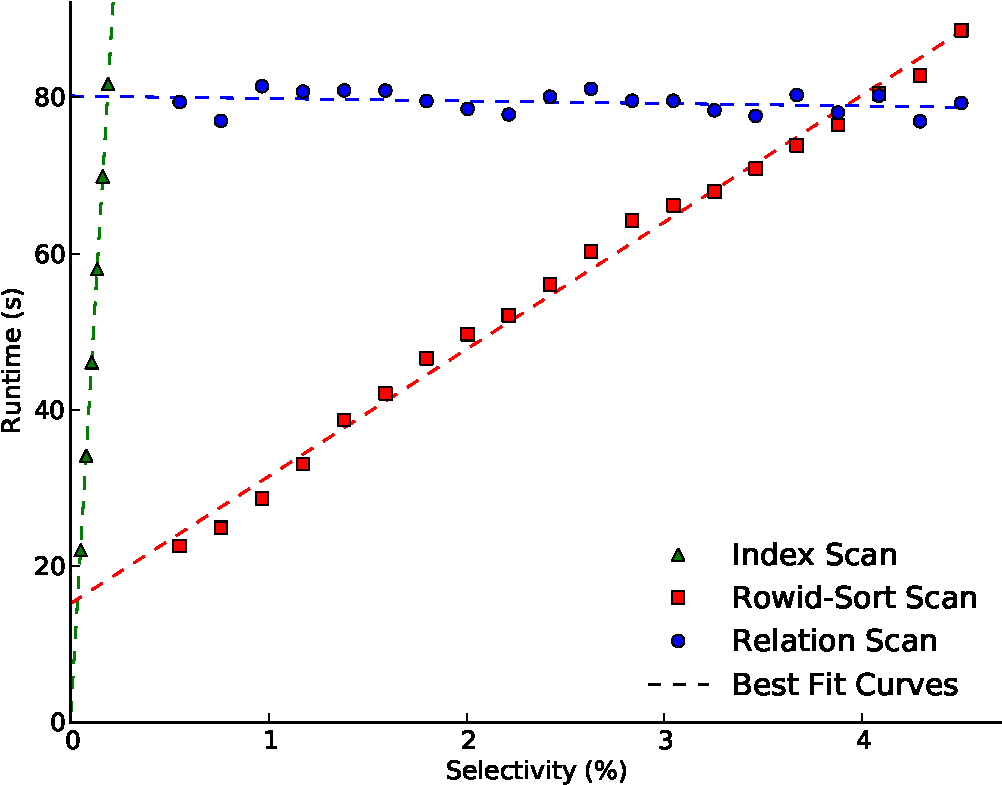
\includegraphics[width=5.0in]{FlashOpti/ScanDisk.pdf}
\caption{ \textbf{Scan operator performance on Disk.} Relation scan outperforms the alternatives at selectivities above 4\%, while index scan is optimal only for vanishingly small selectivities (e.g., single-tuple queries).  Best fit curves drawn for convenience.}
\label{fig:scan-disk}
%}
%\hspace{0.5in}
\end{figure*}
\begin{figure*}
\centering
%\subfigure[Flash SSD.]{
  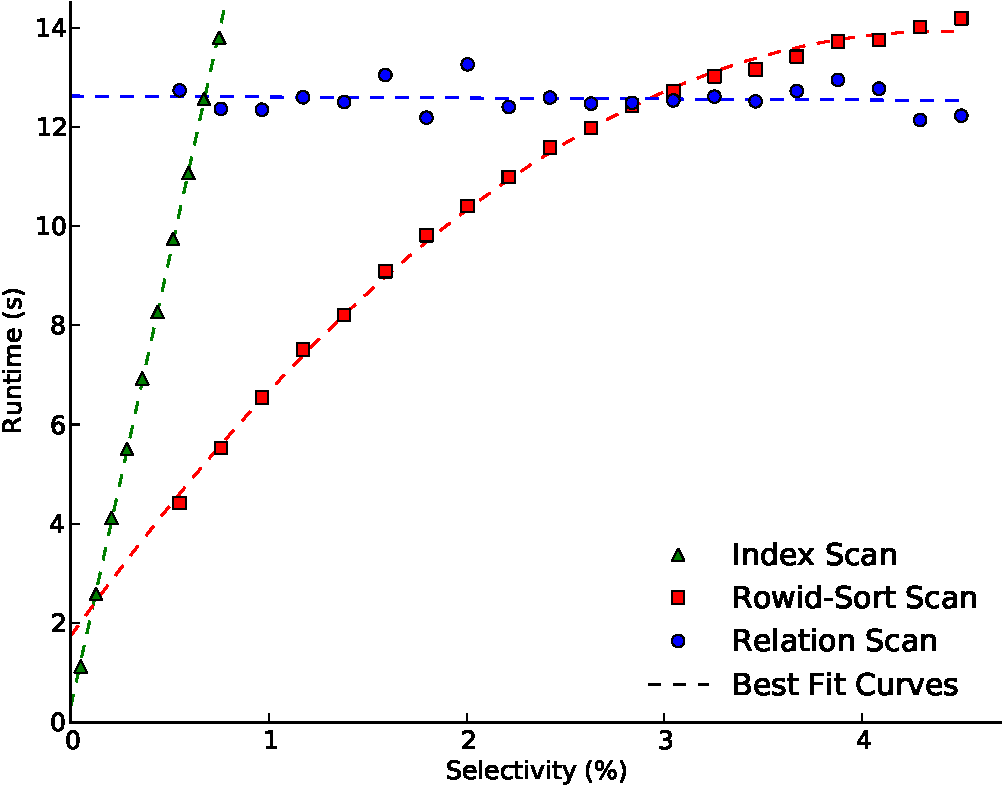
\includegraphics[width=5.0in]{FlashOpti/ScanFlash.pdf}
%}
\caption{ \textbf{Scan operator performance on Flash SSD.} Though both break-even points shift as our intuition suggests, the selectivities where the optimal decision differs between Disk and SSD are so narrow that the difference is inconsequential in practice.  Best fit curves drawn for convenience.}
\label{fig:scan-ssd}
\end{figure*}

I compare the measured performance of the different scan operators as a function of selectivity on SSD and disk.
The objective is to find the break-even points where the optimal scan operator shifts from index scan to rowid-sort scan and finally to relation scan on each device, and the performance impact in regions where this decision differs.
I issue queries for ranges of tuples using a uniformly distributed integer field on a table with 10 million rows, or roughly 2 GB. 
I use a pipelined aggregation function to ensure that no output table is materialized.

Figures~\ref{fig:scan-disk} and~\ref{fig:scan-ssd} report scan runtime on disk and Flash SSD, respectively.
The figures show the measured runtime of each scan (in seconds); lower is better. 
Recall from Section~\ref{sec:FlashOpti:Intro} that classic rules of thumb suggest that, on disk, the break-even point between index and relation scan should occur near 10\% selectivity, and intuition suggests an even higher break-even point for SSD.
Clearly, the conventional wisdom is flawed even for rotating disks; relation scan dominates above selectivities of just 4\% (the trends shown in the figure continue to the right).  
In the intermediate range from about 0.1\% to 4\% selectivity the rowid-sort scan performs best.

However, the more important analysis is to compare the locations of the break-even points across SSD and disk.  
Both crossover points shift in the expected directions.
The slope of the index scan curve is considerably shallower, and the break-even with the relation scan shifts above 0.5\% selectivity.  
Furthermore, the range in which rowid-sort scan is optimal becomes narrower.
Nevertheless, the key take-away is that the range of selectivities for which the optimal scan \emph{differs} across SSD and Disk is vanishingly small.
Only a minute fraction of queries fit into this range, and queries that make the incorrect decision (between disk and Flash) see a small performance impact.
Hence, it is unnecessary for the optimizer to be SSD-aware to choose an effective scan operation.

Whereas these measurements demonstrate my main result, they do not explain why index scans fail to leverage the random access advantage of Flash.  
I turn to this question next. 

\textbf{Analytic results.}
\begin{figure*}
\centering
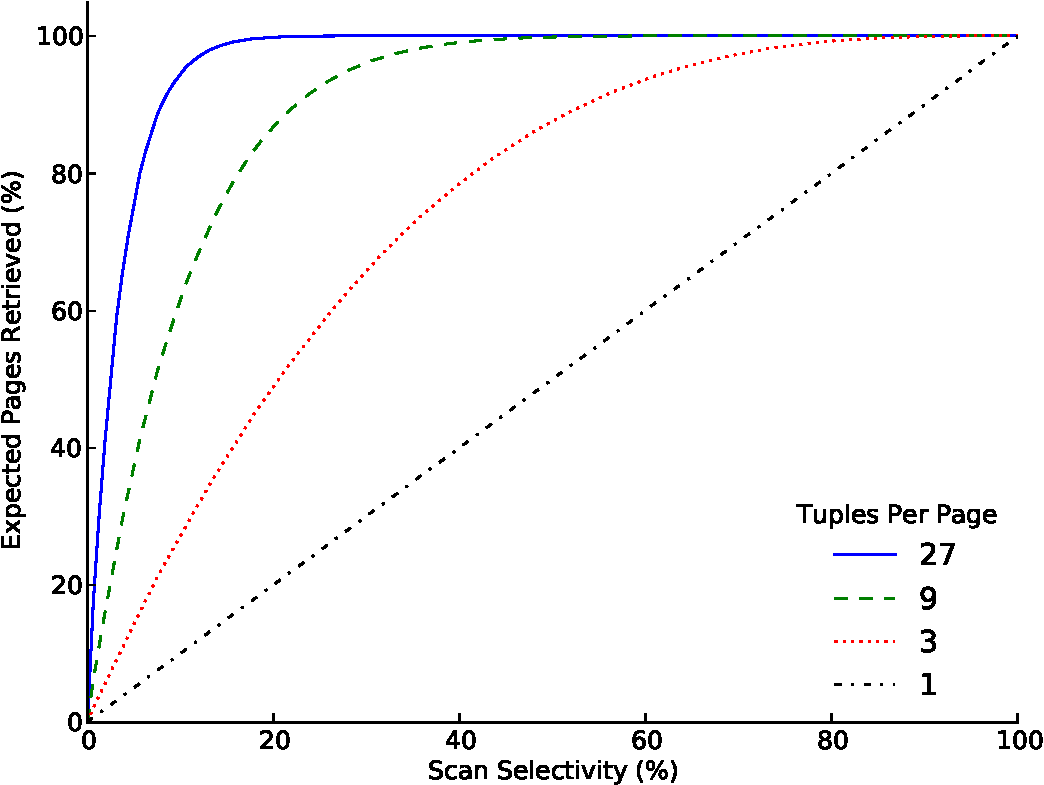
\includegraphics[width=5.0in]{FlashOpti/expectedPagesRet.pdf}
\caption{Index scans touch the majority of pages even at low selectivities.}
\label{figure::analyticScan}
\end{figure*}

The previous results show that index scan underperforms at selectivities far below what the classic 10\% rule of thumb suggests. 
The flaw in the conventional wisdom is that, when there are many tuples per page, the vast majority of \emph{pages} need to be retrieved even if only a few \emph{tuples} are accessed.
When the 10\% rule is applied to page- rather than tuple-selectivity, the guideline is more reasonable.
Yue \emph{et al.} provide an analytical formula for the expected number of pages retrieved given the size of the table, tuples per page, and selectivity \cite{Yue1975}, assuming tuples are randomly distributed among pages (a reasonable assumption given that each table can be clustered on only a single key).
Based on this formula, Figure~\ref{figure::analyticScan} shows the expected percentage of pages retrieved as a function of query selectivity and tuples per page.
When a page contains only a single tuple, clearly, the number of tuples and pages accessed are equal.
However, as the number of tuples per page increases, the expectation on the number of pages that must be retrieved quickly approaches 100\% even at small selectivities.
As a point of reference, given a 4kb page size and neglecting page headers, the Wisconsin Benchmark stores 19 tuples per page while TPC-H's Lineitem and Orders tables store 29 and 30 tuples per page, respectively.

The implication of this result is that, for typical tuple sizes, the vast majority of pages in a relation must be read even if the selectivity is but a few percent.
Hence, with the exception of single-tuple lookups, there are few real-world scenarios where scan performance improves with better random access latency under conventional storage managers that access data in large blocks.
To benefit from low access latency, future devices will need to provide random access at tuple (rather than page) granularity.
Until such devices are available, relation and rowid-sort scans will dominate, with IO bandwidth primarily determining scan performance.

\section{Join Analysis}
\label{sec:FlashOpti:Joins}

I next study the variability in join performance across disk and Flash SSD.  
Again, the objective is to identify cases where the optimal join algorithm for disk consistently results in grossly sub-optimal performance on Flash SSD.
Such scenarios imply that it is important for the optimizer to be SSD aware.

DB2 implements nested loop, sort-merge, and hybrid hash join operators.  
However, DB2 does not support a block nested loop join; its nested loop join performs the join tuple-by-tuple instead of prefetching pages or other blocks, relying on indexes to provide high performance.
Hence, unless the join can be performed in memory, the nested loop grossly underperforms the other two algorithms for ad-hoc queries (those that do not use indexes) regardless of storage device and will not be selected by the query optimizer unless it is the only alternative (e.g., for inequality joins). 
I therefore restrict the investigation to a comparison of sort-merge and hybrid hash joins.

When a clustered index exists for a particular scan or join this index should almost always be used, regardless of the nature of the storage device.  
Hence, I do not include clustered indexes in my analysis.
Furthermore, I evaluate only ad hoc joins.
When indexes are available, the choice of whether or not to use the index is analogous to the choice of which scan operator to use for a simple select query, which is covered by the previous analysis of scans.

Because of the complex interplay between available memory capacity and relation sizes for join optimization \cite{DBLP:journals/vldb/HaasCLS97}, I do not have a specific expectation that one join algorithm will universally outperform another on Flash SSD as opposed to disk.
Rather, I perform a cross-product of experiments over a spectrum of relation sizes and output projectivities using the Wisconsin Benchmark database.  
Haas's model demonstrates the importance of the relative sizes of input relations and main memory capacity on join performance; hence I explore a range of joins that are only slightly larger than available memory (joining two 1.9GB tables) to those that are an order of magnitude larger (joining two 9.7GB tables).   
I vary projectivity, having discovered empirically that it significantly impacts the optimal join algorithm on disk, as it has a strong influence on partition size in hybrid hash joins.
I execute queries with two projectivities: approximately 5\% (achieved by selecting all the integer fields in the Wisconsin Benchmark schema), and approximately 25\% (selecting an integer field and one of the three strings in the schema).
In all experiments, I perform an equijoin on an integer field, and use an aggregation operator to avoid materializing the output.

\begin{figure*}
\centering
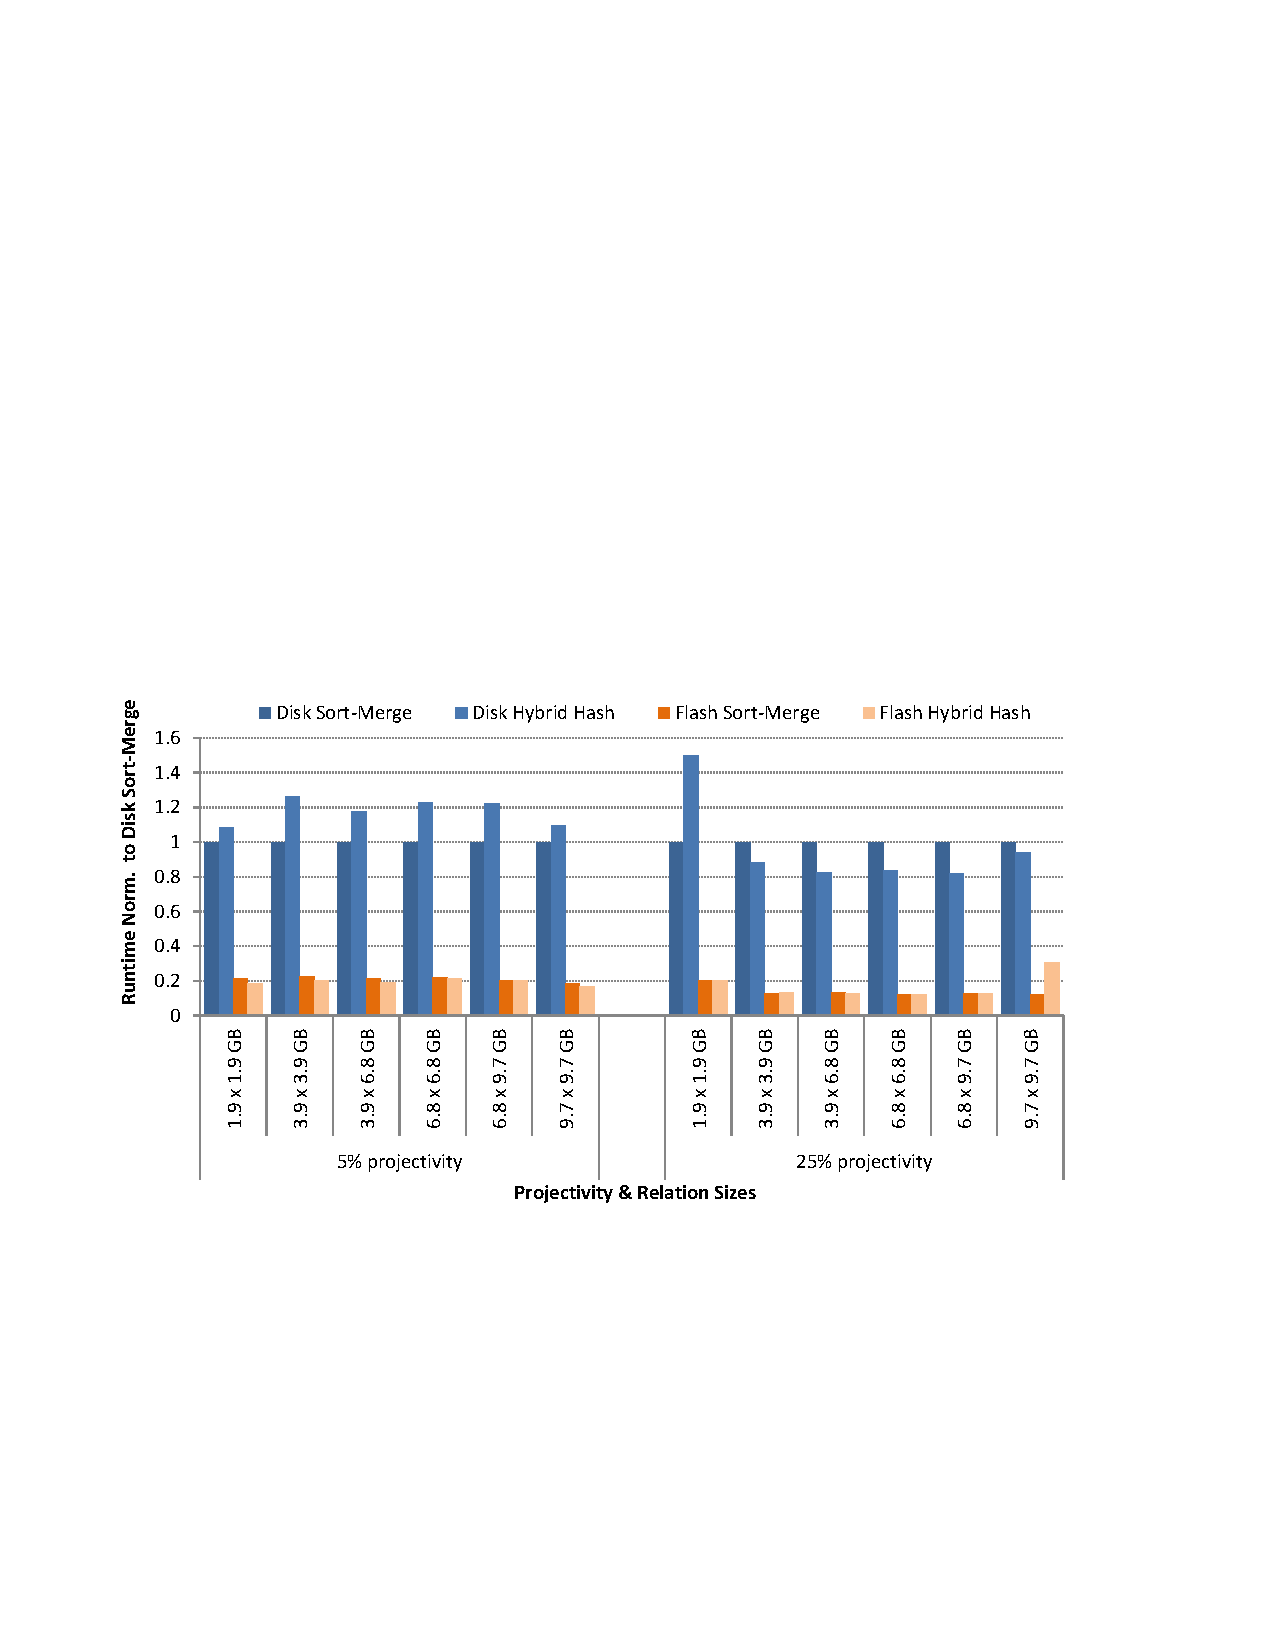
\includegraphics[width=6.0in]{FlashOpti/join.pdf}
\caption{\textbf{Join performance.}  Join runtimes on Flash SSD and Disk, normalized for each join to the runtime of sort-merge on disk.  Though there is significant variability in join algorithm performance on disk, performance variability on SSD is dwarfed by the  6\texttimes~performance advantage of moving data from disk to SSD.}
\label{figure::joins}
\end{figure*}


I report results in graphical form in Figure~\ref{figure::joins} and absolute run times in Table~\ref{table::joins}.
In Figure~\ref{figure::joins}, each group of bars shows the relative performance of sort-merge and hybrid hash joins on disk (darker bars) and Flash SSD (lighter bars), normalized to sort-merge performance on disk.
Lower bars indicate higher performance.
I provide the same data in tabular form to illustrate the runtime scaling trends with respect to relation size, which are obscured by the normalization in the graph.

Two critical results are immediately apparent from the graph.  
First, Flash SSDs typically outperform disk by 5\texttimes~to 6\texttimes~regardless of join algorithm, a margin that is substantially higher than the gap in sequential IO bandwidth, but far smaller than the gap in random IO bandwidth (see Table~\ref{table:DiskCharacteristics}).
Hence, though both join algorithms benefit from the improved random IO performance of SSDs, the benefit is muted compared to the 100\texttimes~device-level potential.
Second, whereas there is significant performance variability between the join algorithms on disk (typically over 20\%), with the exception of a single outlier, the variability is far smaller on Flash SSD (often less than 1\%).
From these results I conclude that although important on disk, the choice of sort-merge vs hybrid hash join on SSD leads to inconsequential performance differences relative to the drastic speedup of shifting data from disk to Flash.
Hence, there is no compelling reason to make the query optimizer SSD-aware; the choice it makes assuming the performance characteristics of a disk will yield near-optimal performance on SSD.

\begin{table*}
\centering
\begin{tabular}{c@{\hspace{12pt}}c@{\hspace{12pt}}c@{\hspace{12pt}}c@{\hspace{1pt}}c@{\hspace{12pt}}c@{\hspace{12pt}}c}
%\begin{tabular}{c  c | c | c | c | c}
  \toprule
	\multirow{2}{*}{Projectivity} 		      & \multirow{2}{*}{Table Sizes} & \multicolumn{2}{c}{Disk}    & &  \multicolumn{2}{c}{Flash SSD}  \\ 
\cmidrule{3-4} \cmidrule{6-7}
	 &  & Sort-merge & Hybrid hash     & &  Sort-merge & Hybrid hash  \\ 
   \midrule
5\%	& 1.9 x 1.9 GB	& 187 	& 202	& & 40		& 34	\\
	& 3.9 x 3.9 GB	& 358	& 451	& & 80		& 72	\\
	& 3.9 x 6.8 GB	& 487	& 574	& & 103	& 93	\\
	& 6.8 x 6.8 GB	& 649	& 795	& & 142	& 140\\
	& 6.8 x 9.7 GB	& 816	& 997	& & 166	& 166\\
	& 9.7 x 9.7 GB	& 1084	& 1189	& & 202	& 183\\
  \midrule
25\% & 1.9 x 1.9 GB	& 236	& 355	& & 48		& 48	\\
	& 3.9 x 3.9 GB	& 751	& 662	& & 97		& 101\\
	& 3.9 x 6.8 GB	& 947	& 781	& & 125	& 122\\
	& 6.8 x 6.8 GB	& 1415	& 1182	& & 174	& 173\\
	& 6.8 x 9.7 GB	& 1581	& 1298	& & 199	& 199\\
	& 9.7 x 9.7 GB	& 2081	& 1955	& & 250	& 634\\
  \bottomrule
\end{tabular}
\caption{\textbf{Absolute join performance.}  Join runtimes in seconds.  Variability in join runtimes is far lower on Flash SSD than on Disk.}
\label{table::joins}
\end{table*}



I highlight two notable outliers in the results.
On disk, the best join algorithm is strongly correlated to query projectivity with the exception of the 1.9GB~\texttimes~1.9GB join at 25\% projectivity.
Because the required hash table size for this join is close to the main memory capacity, I believe that this performance aberration arises due to DB2 selecting poor partition sizes for the join.
Second, on Flash, I observe a large performance difference (over 2\texttimes) between sort-merge and hybrid hash join for the largest test case, a 9.7GB~\texttimes~9.7GB join at 25\% projectivity.
For this query, I observe a long CPU-bound period with negligible IO at the end of the hybrid hash join that does not occur for any of the other hash joins.
Hence, I believe that this performance aberration is unrelated to the type of storage device, and may have arisen due to the methods employed to coax the optimizer to choose this join algorithm.
In any event, neither of these outliers outweigh the broader conclusion that there is no particular need for the query optimizer to be SSD aware.

\section{Related Work}
\label{sec:FlashOpti:RelatedWork}
Previous work studying the applicability of Flash memory in DBMS applications has focused on characterizing Flash, benchmarking specific database operations on Flash, and designing new layouts, data structures, and algorithms for use with Flash.

Both Bouganim \emph{et al.} and Chen \emph{et al.} benchmark the performance of Flash for various IO access patterns \cite{Bouganim09uflip:understanding, Chen2009}.
Bouganim introduces the uFLIP micro-benchmarks and tests their performance on several devices.
Chen introduces another set of micro-benchmarks, concluding that poor random write performance poses a significant barrier to replacing conventional hard disks with Flash SSDs.
While these micro-benchmarks are instructive for understanding database performance, I focus specifically on the performance of existing scan and join operators on SSD and disk.
Others have also benchmarked Flash's performance within the context of DBMS systems.
Lee \emph{et al.} investigate the performance of specific database operations on Flash, including multiversion concurrency control (MVCC), external sort, and hashes \cite{Lee2008}.
Similar to my study, Do \emph{et al.} benchmark ad hoc joins, testing the effects of buffer pool size and page size on performance for both disk and Flash \cite{Do2009}.
Although related to this study, neither of these works look at the specific performance differences between disk and Flash for scans and joins and how this might impact query optimization.

Whereas the above works (and this study) focus on measuring the performance of existing databases and devices, others look ahead to redesign DBMS systems in light of the characteristics of Flash.
Yin \emph{et al.} and Li \emph{et al.} present new index structures, focusing on maintaining performance while using sequential writes to update the index \cite{Yin2009, Li2009}.
Baumann \emph{et al.} investigate Flash's performance alongside a hybrid row-column store referred to as ``Grouping" \cite{Baumann2010}.
Similarly, Tsirogiannis \emph{et al.} use a column store motivated by the PAX layout to create faster scans and joins \cite{Tsirogiannis2009}.

Interestingly, my findings contradict recommendations from many of these studies.
Baumann concludes that SSDs shift optimal query execution towards index-based query plans.
The study bases this conclusion on the observation that asynchronous random reads on Flash are nearly as fast as sequential reads.
Indeed, the arguments made by Baumann are a key component of the intuition laid out in Section~\ref{sec:FlashOpti:Intro} that led me to expect a need for SSD-aware query optimization.
However, the conclusion neglects the observations discussed in Section~\ref{sec:FlashOpti:Scans} demonstrating that queries selecting more than a handful of tuples will likely retrieve the majority of pages in a relation, and thus gain no advantage from fast random IO.
Tsirogiannis introduces a join algorithm that retrieves only the join columns, joins these values, and then retrieves projected rows via a temporary index.
By the previous argument, scanning for projected data should retrieve the majority of data pages, preferring a relation scan, and thus provide comparable advantage on disk and SSD.

Finally, Bausch \emph{et al.} implement asymmetry-aware query optimization in PostgreSQL \cite{BauschPetrov12}.
They calibrate and evaluate their system using the TPC-H benchmark and find substantial improvement.
However, I believe their calibration and evaluation are skewed and lead to false conclusions (their results are insufficient to demonstrate that query optimizers should be SSD-aware).
First, their results show that an external sort of unordered data results results in 95\% random read accesses to disk.
This is indicative of poorly configured memory buffers; external soft algorithms should exhibit almost entirely sequential access patterns.
Furthermore, the results of their calibration (shown in their appendix) differ substantially from expected physical traits.
For example, the relative cost of disk's random access is only $6.8\times$ that of a sequential access, the relative cost of Flash's random read access is $5.6\times$ that of its sequential read access (nearly the same as the relative difference on disk), and Flash's sequential writes are roughly $2.5\times$ \emph{slower} than random writes (sequential writes should be faster).
Using a physically-based model only makes sense if the model is accurate.
I believe the improvement shown is a function of (1) using the total time of 21 queries as the performance and calibration metric instead of arithmetic or geometric mean (query 21 shows improvement of 549\% and has a greater runtime than most other queries), (2) using search-based calibration instead of physically derived optimization parameters (e.g., the cost of a disk seek should be measured directly from the disk, not by fitting the model), and (3) the asymmetric model has seven parameters versus the original model's five; these additional degrees of freedom allow more effective search-based calibration even when using an incorrect optimization model.
I believe that my work demonstrates fundamental principles suggesting that query optimization sees little benefit from SSD-awareness.

\section{Conclusion}
\label{sec:FlashOpti:Conclusion}
Flash-based solid state disks provide an exciting new high-performance alternative to disk drives for database applications.
My investigation of SSD-aware query optimization was motivated by a hope that the drastically improved random IO performance on SSDs would result in a large shift in optimal query plans relative to existing optimizations.
At a minimum, I expected that constants capturing relative IO costs in the optimizer would require update.
This chapter presented evidence that refutes this expectation, instead showing that an SSD-oblivious query optimizer is unlikely to make significant errors in choosing access paths or join algorithms.
Specifically, I demonstrated both empirically and analytically that the range of selectivities for which a scan operation can benefit from SSDs' fast random reads is so narrow that it is inconsequential in practice.
Moreover, measurements of alternative join algorithms reveal that their performance variability is far smaller on SSDs and is dwarfed by the 5\texttimes~to 6\texttimes~performance boost of shifting data to SSD. 
Overall, I conclude that the small and inconsistent performance gains available by making query optimizers SSD-aware are not worth the effort.


 \chapter{Particle Transport and Acceleration}
 \label{chap:Particles}
 \section{Introduction}
\label{Transport Intro}
For reference, some common equations and brief overviews of the three categories of particles will be given in this chapter. The Maxwell equations \eqref{Gauss}--\!\,\eqref{Ampere}, the continuity equation for charge density and current density \eqref{continuity}, the Lorentz force equation \eqref{Lorentz}, Newton's second law of motion \eqref{Newton2}, and the \ac{MHD} approximation of Ohm's Law \eqref{Ohm} are each useful for basic plasma physics. Thorough derivations for these and related equations can be found in several textbooks, including \citet{gombosi98} and \citet{jackson99}.

\begin{subequations}
 \begin{align}
  \nabla\cdot\mathbf{E}&=\frac{\rho_e}{\epsilon_0}&\quad\text{Gauss's Law}
  \label{Gauss}\\
  \nabla\times\mathbf{E}&=-\frac{\partial\mathbf{B}}{\partial t}&\quad\text{Faraday's law of induction}
  \label{Faraday}\\
  \nabla\cdot\mathbf{B}&=0&\quad\text{Gauss's law for magnetism}
  \label{Gauss m}\\
  \nabla\times\mathbf{B}&=\mu_0\mathbf{J}+\mu_0\epsilon_0\frac{\partial\mathbf{E}}{\partial t}&\quad\text{Amp\`{e}re's law}
  \label{Ampere}
 \end{align}
\end{subequations}
\begin{align}
 \nabla\cdot\mathbf{J}&=-\frac{\partial\rho_e}{\partial t}&\quad\text{continuity equation}
 \label{continuity}\\
 \mathbf{F}&=q\left(\mathbf{E}+\mathbf{v}\times\mathbf{B}\right)\quad\text{(N)}&\quad\text{Lorentz force}
 \label{Lorentz}\\
 \mathbf{F}&=m\mathbf{a}\quad\text{(N)}&\quad\text{Newton's 2nd law of motion}
 \label{Newton2}\\
 \mathbf{J}&=\sigma\left(\mathbf{E+v\times B}\right)\quad\text{(A m$^{-2}$)}&\quad\text{Ohm's law}
 \label{Ohm}
\end{align}

In these equations, $\epsilon_0$ is the electric constant (also called the permittivity of free space), $\mu_0$ is the magnetic constant (also called the permeability of free space), $\sigma$ is the electrical conductivity, treated here as a constant, $q$ is the charge, $\rho_e$ is the charge density, $m$ is the mass, $\mathbf{J}$ is the electric current density, and $\mathbf{E}$ and $\mathbf{B}$ are the electric and magnetic fields. $\mathbf{F}$, $\mathbf{v}$, and $\mathbf{a}$ represent force, velocity, and acceleration. 

In \ac{MHD}, the fields are induced by plasma motion, so the fields vary on the same time and length scales as the plasma variables. If high frequency variations in the electric field are not included, and only the non-relativistic regime is considered, the displacement current in Amp\`{e}re's law can be neglected, leading to Equation~\ref{AmpereMHD}.
\begin{align}
 \nabla\times\mathbf{B}&=\mu_0\mathbf{J}&&\quad\text{MHD Amp\`{e}re's law}
 \label{AmpereMHD}
\end{align}
\indent By substituting Equation~\ref{Faraday} and the curl of Equation~\ref{AmpereMHD} into the curl of Equation~\ref{Ohm}, $\mathbf{E}$ and $\mathbf{J}$ can be eliminated to derive the magnetic induction equation \eqref{MHDinduction}. The first term on the right describes the resistive diffusion of the magnetic field in the plasma while the second term describes the convection of the magnetic field by the plasma.
\begin{align}
 \frac{\partial\mathbf{B}}{\partial t}=\frac{1}{\sigma\mu_0}\nabla^2\mathbf{B}+\nabla\times\left(\mathbf{v}\times\mathbf{B}\right)&&\quad\text{magnetic induction equation}
 \label{MHDinduction}
\end{align}

Since Equation~\ref{Gauss m} states that the divergence of the magnetic field vector $\mathbf{B}$ is zero, $\mathbf{B}$ can be written in terms of a vector potential $\mathbf{A}$:
\begin{align}
 \mathbf{B}=\nabla\times\mathbf{A}\quad\text{(T)}.
 \label{B field}
\end{align}

By substituting Equation~\ref{B field} into Equation~\ref{Faraday}, Faraday's law of induction can be written as a quantity with a vanishing curl. Such a quantity can be rewritten as the gradient of a scalar function, the scalar potential $\Phi$, leading to an equation for $\mathbf{E}$ in terms of the potentials $\mathbf{A}$ and $\Phi$:
\begin{align}
 \mathbf{E}=-\nabla\Phi-\frac{\partial\mathbf{A}}{\partial t}\quad\text{(V m$^{-1}$)}.
 \label{E field}
\end{align}

For electrostatics, all derivatives with respect to time are zero. In this case, the divergence of Equation~\ref{E field} combined with Equation~\ref{Gauss} will give the Poisson equation, or in the absence of charges, the Laplace equation:
\begin{align}
 \nabla^2\Phi &= -\frac{\rho_e}{\epsilon_0},&\quad\text{Poisson's equation}
 \label{Poisson}\\
 \nabla^2\Phi &= 0.&\quad\text{Laplace's equation}
 \label{Laplace}
\end{align}

Due to the historical precedent of the symbols used in these and other common equations, a symbol may have different meanings depending on the equation in which it is used (i.e., `E' can represent `electric field' or `energy'). Even though the meaning of the symbol can usually be discerned from the context of the equation, an attempt has been made to use distinct symbols throughout this dissertation, or use subscripts to clarify a symbol's meaning when necessary. In the specific case of `E', the bold font $\mathbf{E}$ is used to represent the electric field vector and $\left|\mathbf{E}\right|$  to represent the magnitude of the electric field. The plain font E is always used here to represent energy.

Particle transport and acceleration are important topics of research in heliophysics. An understanding of the composition and nature of the gas and plasma found in space is vital to the forecasting of space weather. This research focuses on ways to investigate three categories of particles: the solar wind (\S~\ref{Solar Wind}), pickup ions, and energetic particles, as shown in Figure~\ref{fig:H_Distribution}. The following is intended to provide sufficient background for the scope of this dissertation research.
%\begin{figure}
%  \centering
%  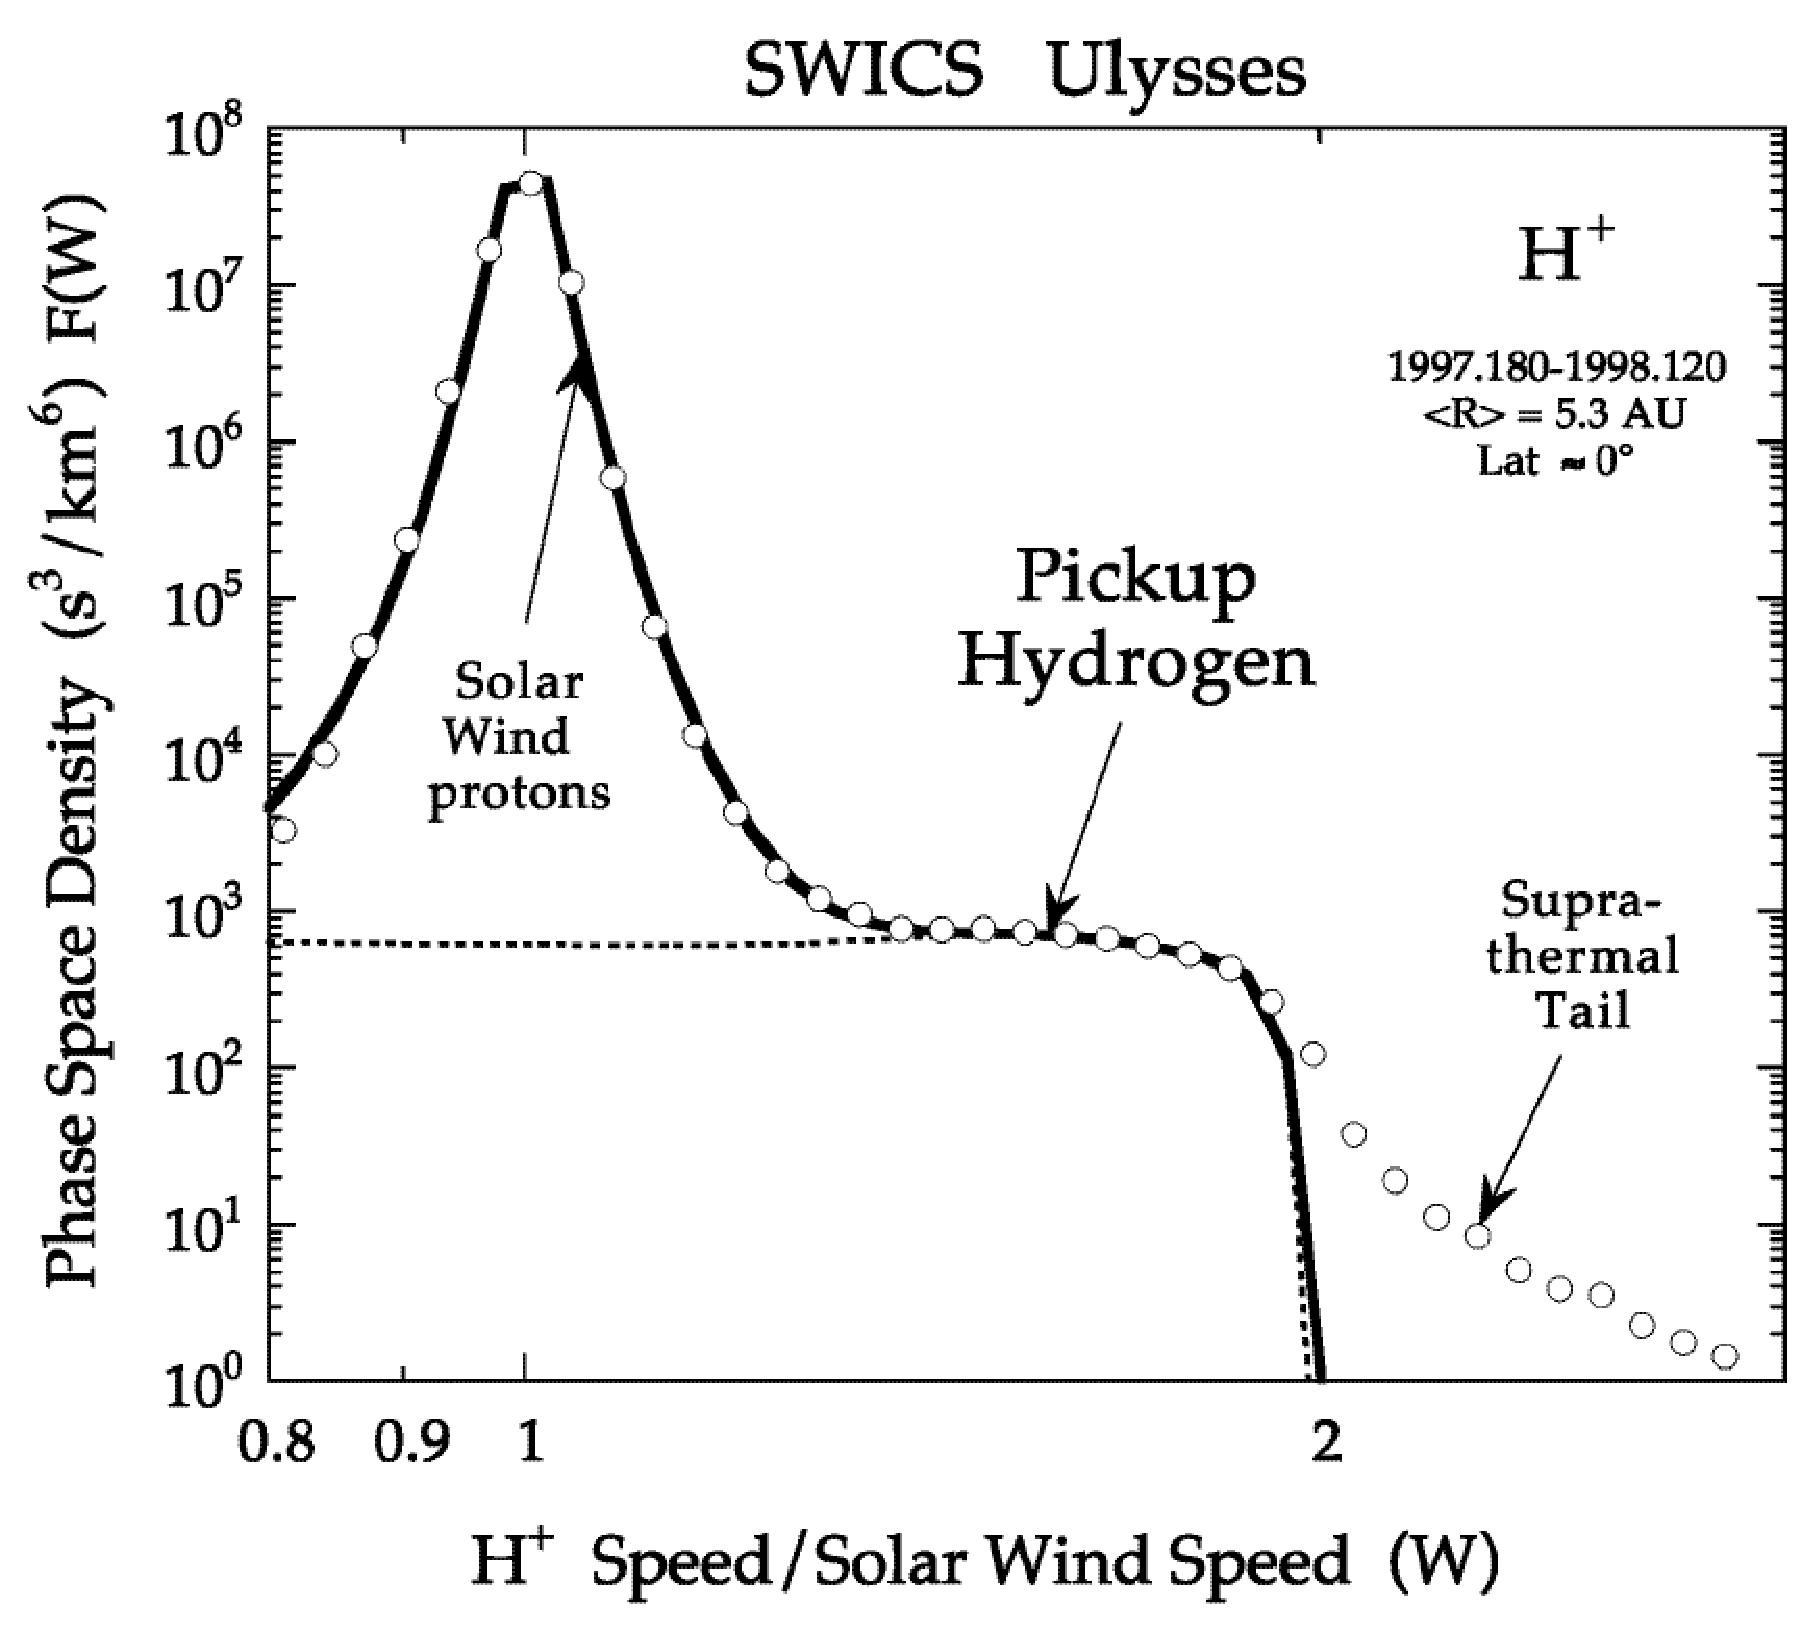
\includegraphics[width=.65\textwidth]{Chap2/H_Distribution}
%  \caption[Example of proton distributions for the quiet solar wind near 5 AU.]{Example of proton distributions for the quiet solar wind near 5 AU. Shown are the bulk distribution of the solar wind, the interstellar pickup ions that drop off at twice the solar wind speed, and the high-energy protons that make up the suprathermal tail. Figure from \citet{gloeckler01b}.}
%  \label{fig:H_Distribution}
%\end{figure}

\section{The Solar Wind}
\label{Solar Wind}

\subsection{Current Knowledge}
\label{SW Current Knowledge}
While he was not the first to postulate its existence, the physics of the solar wind was first explained by Eugene Parker in 1958 \citep{parker58}. Beginning with subsonic speeds close to the Sun, plasma accelerates away from the solar surface and reaches supersonic speeds in the corona. It continues to expand in a radial direction outward until it interacts with the material in interstellar space at the edge of the heliosphere, the Sun's sphere of influence. The wind draws the solar magnetic field along with it, creating spiral-shaped field lines as the Sun rotates \citep{parker59}. Mankind's understanding of the processes that govern the solar wind has increased as spacecraft have taken in situ measurements, but there are still some properties that remain unexplained, such as the precise origin of certain types of wind, as discussed below.

The solar wind travels a distance of one \ac{AU} before reaching Earth's orbit, where most of the current measurements have been taken (Table~\ref{tab:solar wind}). It is generally divided into two components, commonly referred to as the ``fast'' and ``slow'' solar wind. Originally, these terms were used to differentiate the wind by the speed with which it traveled, but more recent studies have shown that the two types of wind are more efficiently distinguished by their charge state composition (e.g., O$^{7+}$/O$^{6+}$) since the plasma can change speeds as it flows through space \citep{geiss95b, gloeckler03a}. Rather than the terms ``fast'' and ``slow'', more appropriate labels are descriptive of the wind's origin: ``coronal hole'' and ``streamer'' wind. These two types of wind are generated by different processes and have different compositions, temperatures, speeds, and origins.
\begin{table}[htbp]
	\centering
		\begin{tabular}{l|c|c}
		                                                               & Coronal Hole Wind & Streamer Wind     \\ \hline
      bulk speed \footnotesize{$\left(\text{km s}^{-1}\right)$}    & 750               & 400               \\ \hline
      thermal speed \footnotesize{$\left(\text{km s}^{-1}\right)$} & 32                & 35                \\ \hline
      H$^+$ density \footnotesize{$\left(\text{cm}^{-3}\right)$}   & 2.5               & 8.7               \\ \hline
      frozen-in temperature \footnotesize{$\left(\text{K}\right)$} & 8 x 10$^5$        & 1.4--1.6 x 10$^6$ \\ \hline

		\end{tabular}
	\caption[Average characteristics of the solar wind at 1 AU.]{Average characteristics of the solar wind at 1 AU. The temperature is derived from the freeze-in temperature of C$^{6+}$/C$^{5+}$, which freezes in near the solar wind source altitude. Data compiled from \citet{vonsteiger95, gloeckler98a, ipavich98, mccomas00, feldman05}.}
	\label{tab:solar wind}
\end{table}

As solar wind ions escape from the photosphere and travel up through the corona, they experience collisions with energetic electrons that ionize them to different degrees. As they travel farther through the corona, continuously accelerating, the density of coronal electrons decreases and the particles experience fewer collisions. When the timescale for ionization or recombination becomes longer than the timescale of the solar wind to expand through a density scale height, the charge state of the ion is said to be ``frozen in,'' branding the ion with the coronal region and electron temperature of its origin \citep{hundhausen68}. The streamer wind has a distinct characteristic of being enriched in elements with a low ($\le$ 10 eV) \ac{FIP} by a factor of 3--4 over the photospheric value. The coronal hole wind does not show this density enhancement, and measurements have revealed abundances of low-\ac{FIP} elements that match ratios in the photosphere \citep{vonsteiger93}. The streamer wind also has a higher and more variable freeze-in temperature than the coronal hole wind. One explanation for this describes solar plasma trapped and heated in large coronal loops that are eventually opened by interchange reconnection, releasing the plasma \citep{gosling95, fisk98, fisk99a}.

The coronal hole wind originates in the open flux regions of the Sun, which contain low-density plasma and concentrations of magnetic flux that are all the same polarity. During solar minimum these regions are clustered around the poles of the Sun, while during solar maximum they appear at all latitudes. Plasma in open flux regions is also released from flux loops, but the high concentration of open flux increases the probability that the loops will open before they can heat and fractionate the plasma. The anti-correlation between freeze-in temperature and solar wind speed shown in Table~\ref{tab:solar wind} can be interpreted in a simplistic way as a sign of different sized loops. The long-lived loops that produce the streamer wind will expand and rise slowly into the corona, where the temperatures are hotter, before being opened \citep{fisk98, fisk01a}. The short-lived loops that yield the coronal hole wind are opened while they are still small and close to the cooler surface \citep{fisk99a, fisk03, wimmer03b}.


\startappendices
 \appendix{Two-Dimensional Crank-Nicolson Scheme for a Uniform Spherical Grid}
 \label{app:CN Scheme}
 This is an example appendix.
For the diffusion process, The equation was solved using a two-dimensional implicit Crank-Nicolson scheme, which is unconditionally stable and second-order accurate in both time and space \citep{crank47}. In the conventional notation, the two-dimensional numerical scheme using central differencing can be written for a uniform Cartesian grid as 
\begin{eqnarray}
\nonumber\left(1+2\mu\right)u^{t+1}_{i,j}-\frac{\mu}{2}\left(u^{t+1}_{i+1,j}+u^{t+1}_{i-1,j}+u^{t+1}_{i,j+1}+u^{t+1}_{i,j-1}\right)\\
=\left(1-2\mu\right)u^{t}_{i,j}+\frac{\mu}{2}\left(u^{t}_{i+1,j}+u^{t}_{i-1,j}+u^{t}_{i,j+1}+u^{t}_{i,j-1}\right),
\end{eqnarray}

\noindent where $u^{t}_{i,j}$ is the value of the parameter undergoing the diffusion ($B_{r}$ in this case) at position $(i, j)$ at time \textit{t}. The von Neumann number on a uniform grid is $\mu=\xi{\Delta}t/\left({\Delta}x\right)^{2}$, where the size of the grid square is $\Delta x$ on each side, and the diffusion coefficient $\xi$ describes the speed at which the mathematical diffusion takes place. When deriving the two-dimensional Crank-Nicolson scheme in spherical coordinates, the von Neumann number is written as $\mu=\xi{\Delta}t/\left(r\Delta\theta\right)^{2}$, where $\Delta\theta=\Delta\phi$, and the cosine is replaced by the central difference of the sine to remain consistent with the discrete nature of the other terms. Care must be taken at the poles, where the central differencing is replaced by forward or backward differencing. To keep second-order accuracy with forward or backward differencing, the series must be carried out to higher-order terms in the derivation. The two-dimensional numerical scheme using central differencing can be written for a uniform spherical grid as
\begin{multline}
\left(1+\mu+\frac{\mu}{\sin^{2}\theta_{i,j}}\right)u^{t+1}_{i,j}-\frac{\mu}{2}\left[1+\frac{\left(\sin\theta_{i+1,j}-\sin\theta_{i-1,j}\right)}{4\sin\theta_{i,j}}\right]u^{t+1}_{i+1,j}\\
 -\frac{\mu}{2}\left[1-\frac{\left(\sin\theta_{i+1,j}-\sin\theta_{i-1,j}\right)}{4\sin\theta_{i,j}}\right]u^{t+1}_{i-1,j}-\frac{\mu}{2}\frac{1}{\sin^{2}\theta_{i,j}}u^{t+1}_{i,j+1}-\frac{\mu}{2}\frac{1}{\sin^{2}\theta_{i,j}}u^{t+1}_{i,j-1}\\
 =\left(1-\mu-\frac{\mu}{\sin^{2}\theta_{i,j}}\right)u^{t+1}_{i,j}+\frac{\mu}{2}\left[1+\frac{\left(\sin\theta_{i+1,j}-\sin\theta_{i-1,j}\right)}{4\sin\theta_{i,j}}\right]u^{t+1}_{i+1,j}\\
 +\frac{\mu}{2}\left[1-\frac{\left(\sin\theta_{i+1,j}-\sin\theta_{i-1,j}\right)}{4\sin\theta_{i,j}}\right]u^{t+1}_{i-1,j}+\frac{\mu}{2}\frac{1}{\sin^{2}\theta_{i,j}}u^{t+1}_{i,j+1}+\frac{\mu}{2}\frac{1}{\sin^{2}\theta_{i,j}}u^{t+1}_{i,j-1}.
 \label{CN Spherical}
\end{multline}

%Although it is unconditionally stable, a marching scheme such as this will depend on the value of $\mu$ for its accuracy. A lower choice of $\mu$ will lead to a more accurate solution at the expense of computational resources (i.e., a smaller time step ${\Delta}t$), while a higher value of $\mu$ will arrive at a solution more rapidly but with less accuracy (a larger time step). In this model, the value of the coefficient $\xi$ describes the speed of the mathematical relaxation and, since it does not describe a physical process, can be chosen arbitrarily. Thus the only restriction for this scheme will lie in keeping $\mu$ small for accuracy and assigning either $\xi$ or ${\Delta}t$. It can be seen that when $\mu$ is held constant, any choice for either $\xi$ or ${\Delta}t$ will lead to the same solution. A value of $\mu=1/4$ was chosen, with an arbitrary time step of ${\Delta}t=0.1$ s, and studied several different grid resolutions, with a grid size of 2.5$^\circ$ x 2.5$^\circ$ (72 x 144 grid spaces) on a uniform spherical grid used for the comparisons in this paper. The relaxation was allowed to continue on a sphere of $r=R_{\sun}$ until the difference in magnetic field magnitude between any cell and its neighbor was of order $10^{-1}{\mu}T$.

 
\startbibliography
 \begin{singlespace} % Bibliography must be single spaced
  \bibliography{References}   % Use the BibTeX file ``References.bib''.
 \end{singlespace}

% An external Abstract that can be printed at the end of the document, 
% for separate submission to Rackham. Comment it out when not needed. - jg
%\startextabstractpage
%{The Title of Your Dissertation}{Your Name}{Chair: Albert Einstein}
%Emerging storage technologies offer an alternative to disk that is durable and allows faster data access.
Flash memory, made popular by mobile devices, provides block access with low latency random reads.
New nonvolatile memories (NVRAM) are expected in upcoming years, presenting DRAM-like performance alongside persistent storage.
Wheres both technologies accelerate data accesses due to increased raw speed, used merely as disk replacements they may fail to achieve their full potentials.
Flash's asymmetric read/write access (i.e., reads execute faster than writes) opens new opportunities to optimize Flash-specific access.
Similarly, NVRAM's low latency persistent accesses allow new designs for high performance failure-resistant applications.

This thesis addresses software and hardware system design for such storage technologies.
First, I investigate analytics query optimization for Flash, expecting Flash's fast random access to require new query planning.
While intuition suggests scan and join selection should shift between disk and Flash, I find that query plans chosen assuming disk are already near-optimal for Flash.
Second, I examine new opportunities for durable, recoverable transaction processing with NVRAM.
Existing disk-based recovery mechanisms impose large software overheads, yet updating data in-place requires frequent device synchronization that limits throughput.
I introduce a new design, \GroupCommit, to amortize synchronization delays over many transactions, increasing throughput at some cost to transaction latency.
Finally, I propose a new framework for persistent programming and memory systems to enable high performance recoverable data structures with NVRAM, extending memory consistency with persistent semantics to introduce \emph{memory persistency}.

%\label{ExtAbstract}

\end{document}
